\chapterimage{images/fragments/fragments.jpg} % Chapter heading image

\chapter{Fragments}
Fragments are an optional layer you can put between your activities and your widgets, designed to help you reconfigure your activities to support screens both large (e.g., tablets) and small (e.g., phones). 

If you regard Android as an MVC architecture, fragments and activities combine to be the controller layer. Fragments serve as a local controller, focused on their set of widgets, populating them from model data, and handling
their events. Activities will serve as more of an orchestration layer, handling cross- fragment communications (e.g., a click in Fragment A needs to cause a change in what is displayed in Fragment B).

This chapter is built from the following resources: \cite{Point2017, TueDao2017, Guide2017, murphymarkl.2017,Gleason2017}.

\section{Design Philopsophy of fragments}
Android introduced fragments in Android 3.0 (API level 11), primarily to support more dynamic and flexible UI designs on large screens, such as tablets. Because a tablet's screen is much larger than that of a handset, there's more room to combine and interchange UI components. Fragments allow such designs without the need for you to manage complex changes to the view hierarchy. By dividing the layout of an activity into fragments, you become able to modify the activity's appearance at runtime and preserve those changes in a back stack that's managed by the activity.

Fragments offer

\begin{itemize}
	\item Modularity: Dividing complex activity code across fragments for better organization and maintenance.
	\item Reusability: Placing behavior or UI parts into fragments that can be shared across multiple activities.
	\item Adaptability: Representing sections of a UI as different fragments and utilizing different layouts depending on screen orientation and size.
\end{itemize}

You should design each fragment as a modular and reusable activity component. That is, because each fragment defines its own layout and its own behaviour with its own life cycle callbacks, you can include one fragment in multiple activities, so you should design for reuse and \textbf{avoid directly manipulating one fragment from another fragment}. This is especially important because a modular fragment allows you to change your fragment combinations for different screen sizes.

\begin{figure}
	\centering
	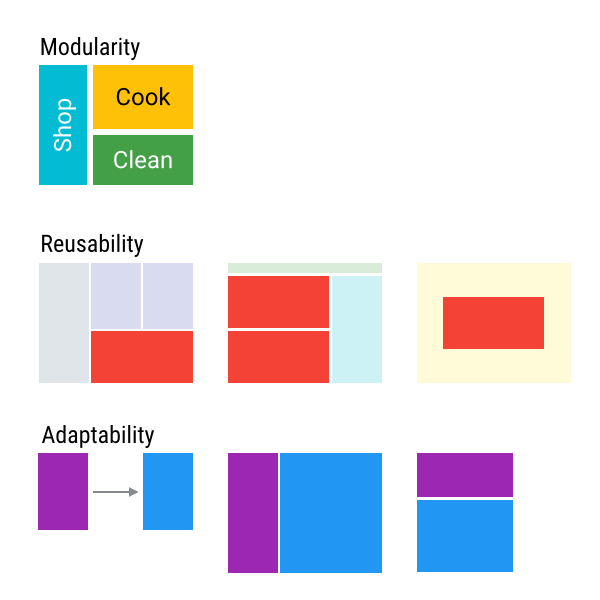
\includegraphics[width=0.7\textwidth]{images/fragments/framgentswhy.png}
	\label{fig:whyfragments}
	\caption{You should design each fragment as a modular, adaptable and reusable component.}
\end{figure}

\section{How to work with activities and fragments}
To explain the use of fragments we will be looking at an example implementation from  \cite{murphymarkl.2017}. You can find the link \href{https://github.com/commonsguy/cw-omnibus/tree/master/Fragments/Static}{here}.

\begin{framed}
	When implementing the exercises for this course you have to use github. Off course you know you do not put every file of your project on the repository. Look how the author of \cite{murphymarkl.2017} have done this on their repository. 
\end{framed}

\subsection{Create a fragment class}

To create a fragment, you must create a subclass of Fragment (or an existing subclass of it). The Fragment class has code that looks a lot like an Activity. It contains callback methods similar to an activity, such as onCreate(), onStart(), onPause(), and onStop().

To provide a layout for a fragment, you must implement the \texttt{onCreateView()} callback method, which the Android system calls when it's time for the fragment to draw its layout. Your implementation of this method must return a \texttt{View} that is the root of your fragment's layout.


\begin{android}
	import android.os.Bundle;
	import android.support.v4.app.Fragment;
	import android.view.LayoutInflater;
	import android.view.ViewGroup;
	
	public class ArticleFragment extends Fragment {
		@Override
		public View onCreateView(LayoutInflater inflater, ViewGroup container,
		Bundle savedInstanceState) {
			// Inflate the layout for this fragment
			return inflater.inflate(R.layout.article_view, container, false);
		}
	}
\end{android}

\subsection{Adding a Fragment (XML)}
To add the fragment, you can
declare the fragment inside the activity's layout file.
	In this case, you can specify layout properties for the fragment as if it were a view. You have to provide the name of the fragment class file.


\begin{xml}
	<LinearLayout xmlns:android="http://schemas.android.com/apk/res/android"
	android:orientation="horizontal"
	android:layout_width="fill_parent"
	android:layout_height="fill_parent">
	
	<fragment android:name="com.example.android.fragments.HeadlinesFragment"
	android:id="@+id/headlines_fragment"
	android:layout_weight="1"
	android:layout_width="0dp"
	android:layout_height="match_parent" />
	
	<fragment android:name="com.example.android.fragments.ArticleFragment"
	android:id="@+id/article_fragment"
	android:layout_weight="2"
	android:layout_width="0dp"
	android:layout_height="match_parent" />
	
	</LinearLayout>
\end{xml}

\begin{android}
	import android.os.Bundle;
	import android.support.v4.app.FragmentActivity;
	
	public class MainActivity extends FragmentActivity {
		@Override
		public void onCreate(Bundle savedInstanceState) {
			super.onCreate(savedInstanceState);
			setContentView(R.layout.news_articles);
		}
	}
\end{android}

\subsection{Adding a Fragment (Programmatically)}
To add the fragment programmatically, you can add the fragment to an existing ViewGroup using FragmentTransaction. 

There are some key concepts which you need to take in mind:
\begin{itemize}
	\item To perform a transaction such as add or remove a fragment, you must use the FragmentManager to create a FragmentTransaction.
	\item You should add the initial fragment(s) to the activity during the activity's onCreate() method.
	\item  Your activity layout must include a container View in which you can insert the fragment. Most of the times this will be an empty FrameLayout.
\end{itemize}

Doing the actual placement, or change or delete:

\begin{android}
	 getSupportFragmentManager().beginTransaction().*
\end{android}

 A simple example can be found \href{https://github.com/commonsguy/cw-omnibus/tree/master/Fragments/Dynamic}{here}.



\subsection{The v4 Support library}
In Android, when using fragments, there are two alternative fragment implementations you can use. One type is the fragment that is provided by the platform version. A platform version corresponds to the version of Android that a user is running. For example, a device running Android 6.0 (SDK Version 23) would be running platform version 23 of the library.
The second type is a support library fragment. When you include a support library, it is added to your project in the same manner as any third-party library. This has two benefits when developing applications for multiple versions of Android.
First, it ensures that you have consistency in your code and functionality across different devices and platform versions. This means that bugs, and fixes, will be more consistent across different versions of Android using these libraries.

Second, when new features are added to the latest version of Android, the Android team will often back-port these features via the support library in order for developers to use on older versions of Android.

\begin{framed}
If you are writing an application that will be targeting multiple versions of Android on multiple devices, you should use support libraries for Fragments. You should also use the support library for any other functionality in your application when available. This is considered a best practice by most senior Android developers and the Core Android team. The only time you might want to use a platform library is if you are, in fact, doing very specialized development for an app that is only targeting one version of Android.
\end{framed}

\section{Fragment Life cycle}
Fragments have lifecycle methods, just like activities do. In fact, they support most
of the same lifecycle methods as activities. You can see an overview in figure \ref{fig:fraglifecycle}.


\begin{figure}
	\centering
	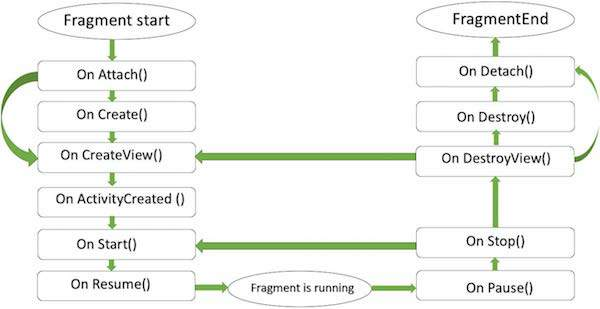
\includegraphics[width=0.8\textwidth]{images/fragments/lifecycle.jpg}
	\caption{Android fragments have their own life cycle very similar to an android activity. Retreived from \cite{Point2017}}
	\label{fig:fraglifecycle}
\end{figure}

The following lifecycle events come into play when you add a fragment:
\begin{description}

\item[onAttach] : When the fragment attaches to its host activity.
\item[onCreate] : When a new fragment instance initializes, which always happens after it attaches to the host — fragments are a bit like viruses.
\item[onCreateView] : When a fragment creates its portion of the view hierarchy, which is added to its activity’s view hierarchy.
\item[onActivityCreated]: When the fragment’s activity has finished its own onCreate event.
\item[onStart] : When the fragment is visible; a fragment starts only after its activity starts and often starts immediately after its activity does.
\item[onResume] : When the fragment is visible and interactable; a fragment resumes only after its activity resumes and often resumes immediately after the activity does.
\item[onPause] : When the fragment is no longer interactable; this occurs when either the fragment is about to be removed or replaced or when the fragment’s activity pauses.
\item[onStop] : When the fragment is no longer visible; this occurs either after the fragment is about to be removed or replaced or when the fragment’s activity stops.
\item[onDestroyView] : When the view and related resources created in onCreateView are removed from the activity’s view hierarchy and destroyed.
\item[onDestroy] : When the fragment does its final clean up.
\item[onDetach] : When the fragment is detached from its activity.
\end{description}
Almost the same rules apply for fragments as do for activities. It is up to the reader to look when each life cycle method is called and when to use it. 

\section{Communication with other Fragments and Activities}

Often you will want one Fragment to communicate with another, for example to change the content based on a user event. All Fragment-to-Fragment communication is done through the associated Activity. 
\begin{framed}
Two Fragments should never communicate directly.
\end{framed}
To allow a Fragment to communicate up to its Activity, you can define an interface in the Fragment class and implement it within the Activity. The Fragment captures the interface implementation during its onAttach() lifecycle method and can then call the Interface methods in order to communicate with the Activity. This way the Fragment can deliver messages to the activity by calling the interface method with a callback instance of the interface defined. 

\section{Communicating from the Activity to the Fragment}
The host activity can deliver messages to a fragment by capturing the Fragment instance with \texttt{findFragmentById()}, then directly call the fragment's public methods.


\section{Exercises}
\begin{exercise}
	Refactor the application you made in exercise \ref{ex:act1} and exercise \ref{ex:act2} in such a way that Fragments are used. You can decide yourself if you prefer dynamic of static fragment setup.
\end{exercise}

\begin{exercise}
	Refactor the application you made in exercise \ref{ex:dotpict}. Your application should:
	\begin{enumerate}
		\item run on large and small devices
		\item landscape and portrait mode
		\item have a layout where the toolbox (tools for drawing your dotpict) is in a fragment, and the drawing itself in another fragment
		\item apply dual pane mode, and single pane mode depending on the orientation or screen size of the device.
	\end{enumerate}
\end{exercise}